% !TeX program = pdflatex
\documentclass[a4paper, twocolumn, 10pt]{article}

\usepackage[a4paper, top=2cm, bottom=2cm, left=1.5cm, right=1.5cm]{geometry}
\usepackage[utf8]{inputenc}
\usepackage[T1]{fontenc}
\usepackage[english]{babel}
\usepackage{mathptmx}
\usepackage{enumitem}
\setlist[itemize]{label=-, noitemsep, topsep=0pt}
\usepackage{amsmath}
\usepackage{booktabs}
\usepackage{graphicx}
\usepackage{titlesec}
\usepackage{url}
\usepackage{abstract}

\titleformat{\section}{\large\bfseries\uppercase}{\thesection.}{1em}{}
\titleformat{\subsection}{\normalsize\bfseries}{\thesubsection.}{1em}{}

\title{\textbf{Continuous Control for Cart-Pole Swingup with Proximal Policy Optimization}}
\author{
    Varun Karthik \\
    \textit{ASU ID: 1234608702} \\[0.5em]
    \textit{Course: EEE598 -- Reinforcement Learning in Robotics} \\
    \textit{November 29, 2025}
}
\date{}

\begin{document}

\maketitle

\begin{abstract}
In this assignment I apply Reinforcement Learning (RL) to the continuous-control Cart-Pole Swingup task from the DeepMind Control Suite. I implement an Actor--Critic agent using Proximal Policy Optimization (PPO) in Stable-Baselines3 and train it for 100\,000 environment steps on the \texttt{dm\_control/cartpole-swingup} environment. To study reproducibility, I train three policies with different random seeds (0, 1, 2) and evaluate each on a held-out evaluation seed (10). The agent reliably improves during training, but the final performance varies across seeds: one run underperforms while the others reach high returns. On average, the evaluation score is about 467 with large variability across seeds, showing both the effectiveness and sensitivity of PPO on this task.
\end{abstract}

\section{Introduction}
The Cart-Pole Swingup task is a standard benchmark for continuous-control methods in robotics. Unlike the classic balancing version, the pole starts hanging downward and must first be swung up before it can be stabilized. This makes the problem more challenging and a good testbed for modern RL algorithms.

The environment I use is \texttt{cartpole-swingup} from the DeepMind Control Suite (DMC) \cite{tassa2018deepmind}. It exposes a continuous action space, so the agent must output real-valued forces rather than discrete left/right actions. To solve this, I use Proximal Policy Optimization (PPO) \cite{schulman2017proximal}, a popular Actor--Critic method that has shown strong performance on many continuous-control tasks.

\section{Methodology}

\subsection{PPO as an Actor--Critic Method}
PPO is an on-policy Actor--Critic algorithm. It maintains two neural networks:
\begin{itemize}
    \item \textbf{Actor (policy):} maps the current observation to a Gaussian distribution over the continuous action (force on the cart).
    \item \textbf{Critic (value function):} estimates the expected return for a state and is used to compute advantage estimates.
\end{itemize}

Instead of directly maximizing the policy gradient, PPO optimizes a clipped surrogate objective that constrains how far the new policy can move from the old one. This simple clipping mechanism stabilizes learning and avoids overly aggressive updates.

\subsection{Implementation Details}
I implement the agent using the \texttt{Stable-Baselines3} PPO class with the \texttt{MultiInputPolicy}. The \texttt{Shimmy} library exposes the DeepMind Control Suite task as a Gymnasium environment with ID \texttt{dm\_control/cartpole-swingup}. I wrap the environment with a \texttt{Monitor} to log episode returns and lengths for plotting.

The DMC environment returns observations as a small dictionary of position and velocity features. The \texttt{MultiInputPolicy} automatically builds a multilayer perceptron that processes these features and outputs the mean of a Gaussian action distribution. A learned log-standard-deviation parameter controls the exploration noise.

\subsection{Hyperparameters}
Table~\ref{tab:hyperparams} lists the main hyperparameters. I follow typical PPO defaults and do not perform extensive tuning, since the goal of the assignment is to implement and evaluate a reasonable actor--critic method rather than to maximize final score.

\begin{table}[h]
\centering
\caption{Training and evaluation hyperparameters.}
\label{tab:hyperparams}
\begin{tabular}{ll}
\toprule
\textbf{Parameter} & \textbf{Value} \\
\midrule
Algorithm & PPO (clip) \\
Policy type & MultiInputPolicy (MLP) \\
Total timesteps & 100\,000 \\
Learning rate & $3 \times 10^{-4}$ \\
Discount factor $\gamma$ & $0.99$ \\
Batch size & 64 \\
Training seeds & 3 (0, 1, 2) \\
Evaluation seed & 10 \\
Eval episodes per seed & 10 \\
\bottomrule
\end{tabular}
\end{table}

\section{Experimental Setup}
For each training seed $s \in \{0,1,2\}$ I create a fresh environment, initialize PPO with that seed, and train for 100\,000 environment steps. The \texttt{Monitor} wrapper records the return and length of every episode. After training, I smooth each learning curve with a moving average and then compute the mean and standard deviation across seeds.

To test generalization, I reload each trained policy and evaluate it on a held-out evaluation seed (10). For each policy I run 10 evaluation episodes and record the mean and standard deviation of the return. These statistics are used to construct two plots: a learning curve with a training and evaluation band, and a per-seed evaluation summary.

\section{Results}

\subsection{Learning Curve}
Figure~\ref{fig:learning_curve} shows the training performance. The solid blue line is the mean episode return across the three training seeds, and the shaded blue region is $\pm 1$ standard deviation. At the start, the return is low and corresponds to almost random behaviour. Between roughly 20\,000 and 40\,000 steps the curve rises quickly, indicating that the agent has discovered a swing-up and balancing strategy. After about 80\,000 steps the mean return approaches 500, although the variance increases near the end because one seed learns more slowly than the others.

The dashed line in Figure~\ref{fig:learning_curve} marks the average evaluation performance on the unseen seed 10, and the orange band shows the across-seed standard deviation. The evaluation band overlaps the later part of the training curve but is quite wide, which already hints at strong seed-to-seed variability.

\subsection{Evaluation Across Seeds}
Figure~\ref{fig:eval_summary} focuses on the evaluation results per training seed. Each bar shows the mean return over 10 episodes for that seed, with error bars indicating the within-seed standard deviation. Seed 0 reaches a moderate score (around 270), seed 1 performs better (around 420), and seed 2 achieves a high score (around 710). Averaging these three means gives an overall evaluation performance of about 467 with an across-seed standard deviation of roughly 224.

These numbers confirm that PPO can learn a strong controller for Cart-Pole Swingup, but they also show that the final policy quality depends strongly on the random seed and stochasticity during training.

\begin{figure}[htbp]
    \centering
    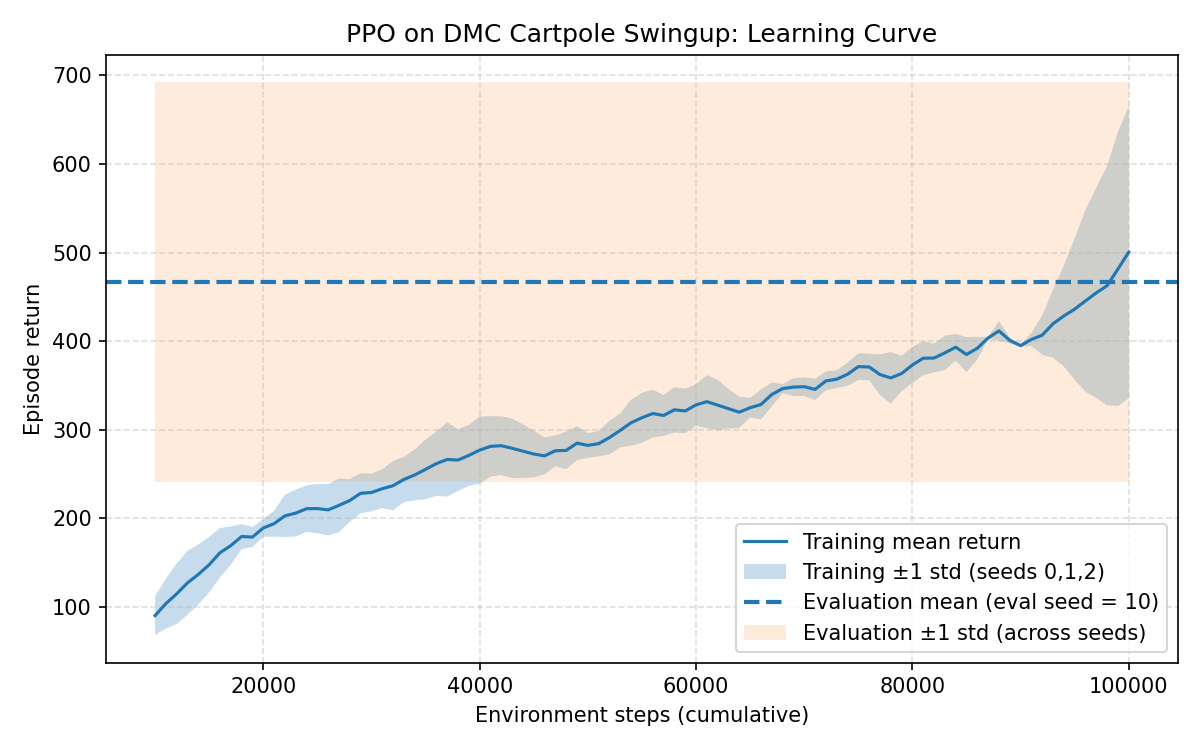
\includegraphics[width=\linewidth]{../rl_results/plots/learning_curve.png}
    \caption{Learning curve of PPO on Cart-Pole Swingup. The blue line is the mean training return across seeds 0, 1, and 2; the blue band is $\pm 1$ standard deviation. The dashed line and orange band show the mean and $\pm 1$ standard deviation of evaluation performance on seed 10.}
    \label{fig:learning_curve}
\end{figure}

\begin{figure}[htbp]
    \centering
    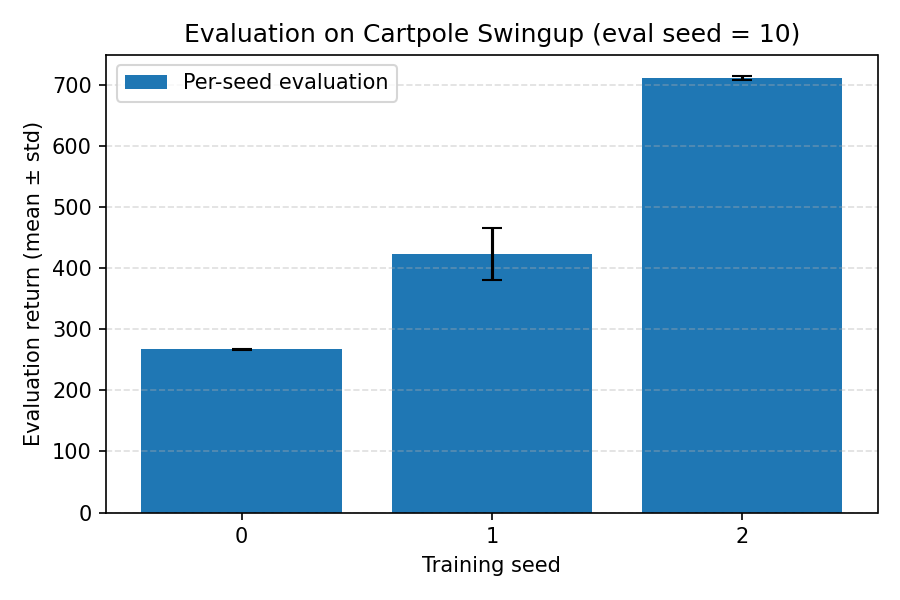
\includegraphics[width=\linewidth]{../rl_results/plots/evaluation_summary.png}
    \caption{Evaluation summary on Cart-Pole Swingup for the held-out seed 10. Each bar shows the mean return over 10 evaluation episodes for one training seed; error bars show within-seed standard deviation.}
    \label{fig:eval_summary}
\end{figure}

\section{Conclusion}
In this assignment I applied PPO, an Actor--Critic algorithm, to the continuous Cart-Pole Swingup task using the DeepMind Control Suite. Training three seeds for 100\,000 steps each leads to good average performance, and the agent learns to swing up and balance the pole. At the same time, the gap between the best and worst seeds is large, so reporting both mean and variance across runs is important. In future work, I could explore longer training, hyperparameter tuning, or alternative algorithms such as SAC or TD3 to reduce this variability.

\begin{thebibliography}{9}

\bibitem{tassa2018deepmind}
Y.~Tassa \textit{et al.}, ``DeepMind Control Suite,'' \textit{arXiv preprint arXiv:1801.00690}, 2018.

\bibitem{schulman2017proximal}
J.~Schulman, F.~Wolski, P.~Dhariwal, A.~Radford, and O.~Klimov, ``Proximal Policy Optimization Algorithms,'' \textit{arXiv preprint arXiv:1707.06347}, 2017.

\bibitem{barto1983neuronlike}
A.~G. Barto, R.~S. Sutton, and C.~W. Anderson, ``Neuronlike adaptive elements that can solve difficult learning control problems,'' \textit{IEEE Transactions on Systems, Man, and Cybernetics}, 1983.

\end{thebibliography}

\end{document}
